\documentclass[12pt]{article}
\usepackage{minted}
\usepackage{geometry}
\usepackage{fontspec}
\usepackage{xeCJK}
\usepackage{setspace}
\usepackage[protrusion=false]{microtype}
\usepackage{graphicx}


\doublespacing

% 本文フォント
\setmainfont{Noto Serif CJK JP}
\setCJKmainfont{Noto Serif CJK JP}

% 等幅フォント
\setmonofont[
  Scale=0.85
]{Noto Mono}

\usemintedstyle{vs}


\geometry{margin=2.5cm}

\title{作業報告書 (YYYY年MM月DD日)}
\author{XX工学科 XX-XXX XXXX}

\begin{document}

\maketitle

\section{作業内容}
GitHub Actionsを使用して、latexで書かれたレポートを自動でPDF化する仕組みを構築した。\\

\section{作業項目}
実装しました。
コードのシンタックスハイライトが効いていることを確認するため、プログラムの例を以下に示す。
ハローワールドを表示するC言語のコードである。

\begin{minted}[fontsize=\small,baselinestretch=1,frame=single,tabsize=4]{c}
#include <stdio.h>

int main() {
    printf("Hello, World!\n");
    return 0;
}

\end{minted}

そして、なんの関係もないが、今回使用した回路図をFigure1に示す。画像ファイルを埋め込めているかの確認のためである。\\
ラズベリーパイを使った回路図である。Kicadというソフトで作成した。

\begin{figure}[htbp]
  \centering
  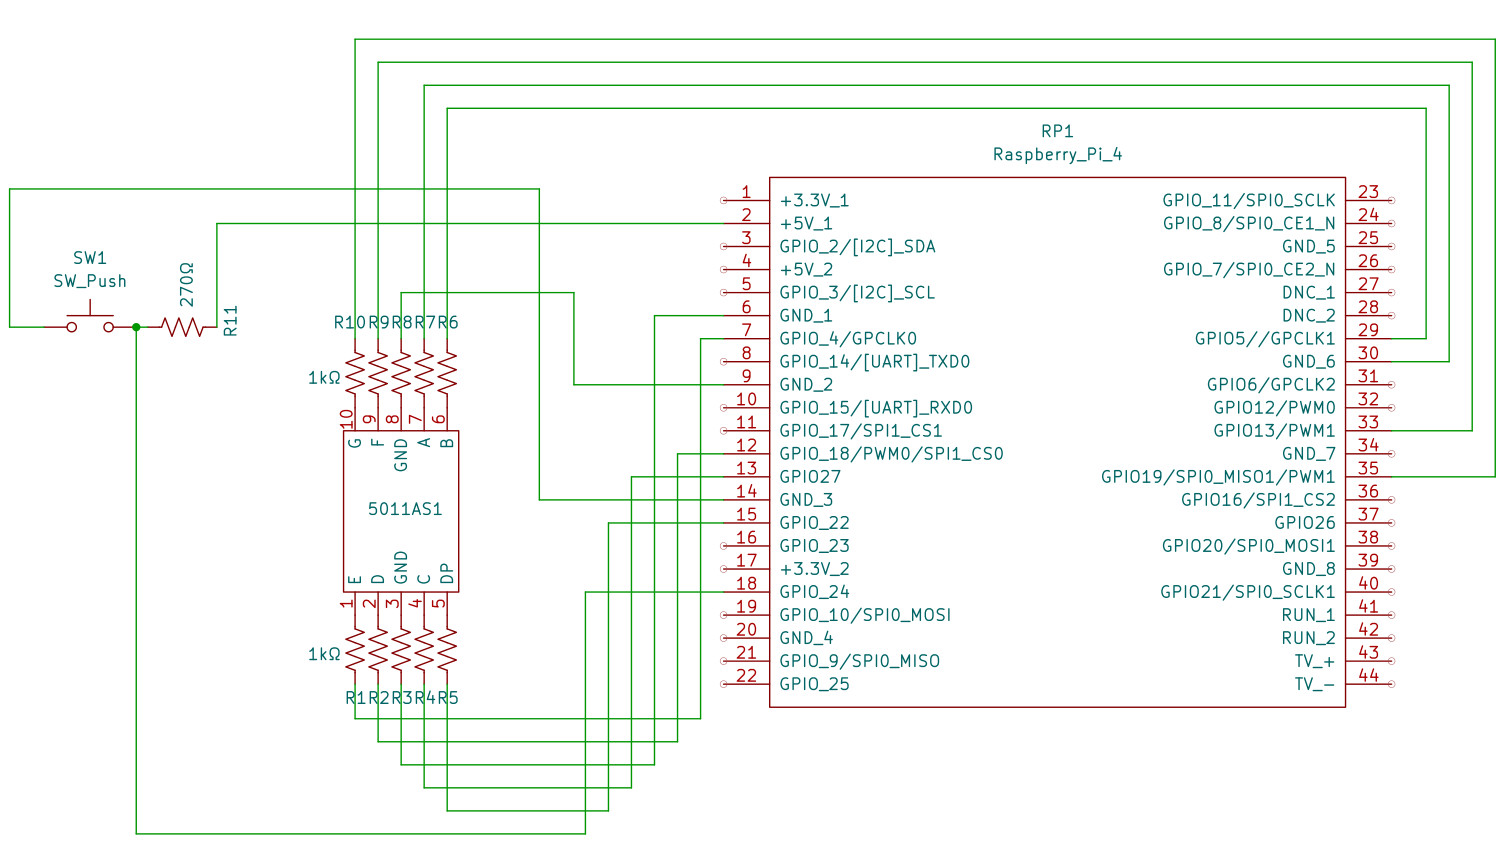
\includegraphics[width=0.8\linewidth]{images/circuit.png}
  \caption{使用した回路図}
  \label{fig:example}
\end{figure}


\noindent
-作業時間\\
    XX分\\
-報告書作成時間\\
    XX分

\end{document}
